% *********************************************************************
% © 2010–2026 Jeremy Sylvestre
%
% Permission is granted to copy, distribute and/or modify this document
% under the terms of the GNU Free Documentation License, Version 1.3 or
% any later version published by the Free Software Foundation; with no
% Invariant Sections, no Front-Cover Texts, and no Back-Cover Texts. A
% copy of the license is included in the appendix entitled “GNU Free
% Documentation License” that appears in the output document of this
% PreTeXt source code. All trademarks™ are the registered® marks of
% their respective owners.
%
% *********************************************************************

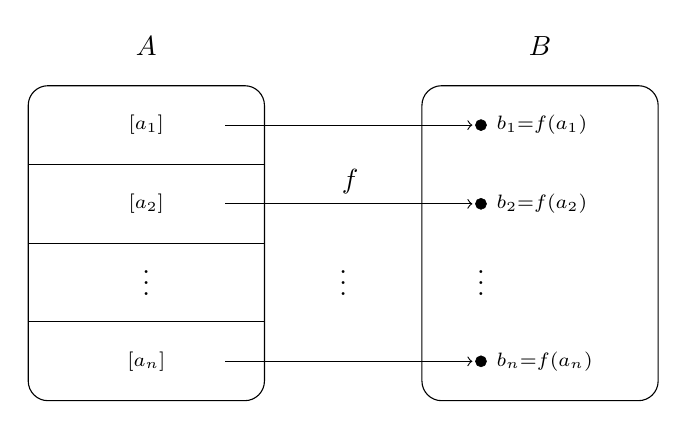
\begin{tikzpicture}[
	vertex/.style={ circle, draw, very thin, fill, inner sep=0pt, minimum size=4pt },
	vertexg/.style={ black!40!white, circle, draw, very thin, fill, inner sep=0pt, minimum size=4pt },
	vertexo/.style={ circle, draw, very thin, inner sep=0pt, minimum size=4pt }
]

\draw (2.75,4) -- (0.25,4)
	arc (90:180:0.25cm) -- (0,0.25)
	arc (180:270:0.25cm) -- (2.75,0)
	arc (270:360:0.25cm) -- (3,3.75)
	arc (0:90:0.25cm);
\node at (1.5,4.5) {$A$};
\draw (0,3) -- (3,3);
\draw (0,2) -- (3,2);
\node at (1.5,1.6) {$\vdots$};
\draw (0,1) -- (3,1);
\node at (1.5,3.5) (a1) {$\scriptstyle [a_1]$};
\node at (1.5,2.5) (a2) {$\scriptstyle [a_2]$};
\node at (1.5,0.5) (ar) {$\scriptstyle [a_n]$};
%		\draw[dashed] (a1.east) -- (0.5,3.5);
%		\draw[dashed] (a2.east) -- (0.5,2.5);
%		\draw[dashed] (ar.east) -- (0.5,0.5);
\draw (7.75,4) -- (5.25,4)
	arc (90:180:0.25cm) -- (5,0.25)
	arc (180:270:0.25cm) -- (7.75,0)
	arc (270:360:0.25cm) -- (8,3.75)
	arc (0:90:0.25cm);
\node at (6.5,4.5) {$B$};
\node at (5.75,3.5) (b1) [vertex,label=right:{$\scriptstyle b_1 = f(a_1)$}] {};
\draw[->,shorten >=1pt] (2.5,3.5) to (b1);
\node at (5.75,2.5) (b2) [vertex,label=right:{$\scriptstyle b_2 = f(a_2)$}] {};
\draw[->,shorten >=1pt] (2.5,2.5) to node[above] {$f$} (b2);
\node at (5.75,0.5) (br) [vertex,label=right:{$\scriptstyle b_n = f(a_n)$}] {};
\draw[->,shorten >=1pt] (2.5,0.5) to (br);
\node at (4,1.6) {$\vdots$};
\node at (5.75,1.6) {$\vdots$};

\end{tikzpicture}
